% *****************************************************************************
%
%        FASThesis Manual
%        (FASThesis Class File Documentation)
%
%        Faculty of Applied Sciences
%        University of West Bohemia
%
%        Manual & Explanatory Document
%        Copyright (c) 2022-2024 Kamil Ekštein, Dept. of Computer Science
%        and Engineering, Faculty of Applied Sciences, UWB
%
%        Version:  0.93
%		 Encoding: UTF-8
%		 TeXer:    pdflatex
%
%        Last modification on 14-Feb-2024 by KE
%
% *****************************************************************************

% _____________________________________________________________________________
%
%
%	     DOCUMENT HEADER
%
% _____________________________________________________________________________
%
\documentclass[english, ba, kiv, he, iso690numb, pdf, viewonly]{fasthesis}
\usepackage{booktabs}
\usepackage{siunitx}
\usepackage{amsmath}
\usepackage[htt]{hyphenat}
\usepackage{csquotes}
\usepackage{caption}
\usepackage{tabularx}
\usepackage{forest}
\hyphenation{vy-tvá-ře-ním}
\DeclareTextFontCommand{\mytexttt}{\ttfamily\hyphenchar\font=45\relax}


\title{Automatic Creation of Summaries of Historical Documents}
%\worktypespec{Technická zpráva}% <== this command is only applicable if 'oth' switch is used above
\author{Václav}{Tran}{}{}
\supervisor{Doc. Ing. Pavel Král, Ph.D.}
\stagworkid{96995}% <== the unique identifier of the work in the STAG information system
% \auxfrontmattercontent{% <== this command only makes sense if 'oth' switch is used above
	% \section*{Test}%
	% Tento text bude vložen do front matteru\dots
% }
\assignment{zadani.pdf}
%\signdate{14th}{03}{2024}{V Plzni}% <== the longest local name in the Czech Rep.
\signdate{14th}{03}{2024}{In Pilsen}% <== the longest local name in the Czech Rep.

\addbibresource{manual.bib}% <== the file with the bibliographical database to be used throughout the text
% _____________________________________________________________________________
%
%
%	     DOCUMENT FRONTMATTER TEXTS
%
% _____________________________________________________________________________
%
\abstract{In the domain of automatic text summarization, neural networks show promising performances. This thesis probes into the task of automatic summarization of Czech historical documents, a largely unexplored niche area with a scant amount of datasets available. To evaluate and improve the performance of our methods, we created our own dataset constructed from a corpus of historical documents. Then we fine-tuned and utilized Transformer-based models Mistral 7B and mT5. We also implemented and evaluated a method, which we refer to as Translation-Summarization-Translation, where we utilize state-of-the-art machine translation and English summarization methods to generate Czech summaries. The performance of these methods set a new baseline for the task of summarizing Czech historical documents.}
% *** English abstract ***
%upravit prvni vetu
{Neuronové síťě dnes dosahují výborných výsledků ve světě automatického vytváření souhrnu dokumentů či textů. Tato bakalářská práce se zabývá automatickým vytvářením souhrnů českých historických dokumentů, což je téma, které není příliš prozkoumané. Pro vyhodnocení a zlepšení výkonu našich metod jsme vytvořili vlastní dataset ze sady historických dokumentů. Poté jsme natrénovali a využili modely Mistral 7B a mT5, které jsou založené na architektuře Transformer. Navíc jsme implementovali a vyohodnotili přístup, který kombinuje nejnovější metody strojového překladu a metody pro automatické vytváření souhrnu textu v angličtině. Tuto metodu označujeme jako Translation-Summarizaton-Translation. Výsledky zmiňovaných metod představují nový základ pro úkol automatické sumarizace českých historických dokumentů.}


\keywords{Neural network, Artificial intelligence, Text summarization, Czech historical documents}
% _____________________________________________________________________________
%
%        ACKNOWLEDGEMENT
% _____________________________________________________________________________
%
\acknowledgement{
I would like to thank my thesis advisor Doc. Ing. Pavel Král, Ph.D. for their constant support and help.

I would also like to thank everyone, who supported me throughout the creation of this Bachelor thesis, including Zach for checking my work for grammatical errors.

Computational resources were provided by the e-INFRA CZ project (ID:90254),
supported by the Ministry of Education, Youth and Sports of the Czech Republic.
}
% _____________________________________________________________________________
%
%
%	     DOCUMENT TEXT BEGINNING
%
% _____________________________________________________________________________
%
\begin{document}
\frontpages[tm] % or notm if the `trademark' declaration is not needed
\tableofcontents
% 
% -x---- ADDITIONAL COLOUR DEFINITIONS ----------------------------------------
%
\makeatletter%
\ifx\FASThesis@style\c@fullcolor%
	\definecolor{fascolor}{cmyk}{0.06, 0.27, 1.0, 0.12}%
	\definecolor{fascolordk}{cmyk}{0.05, 0.28, 1.0, 0.24}%
\else%
	\definecolor{fascolor}{cmyk}{0, 0, 0, 0.6}%
	\definecolor{fascolordk}{cmyk}{0, 0, 0, 0.75}%
\fi%
\makeatother%
\lstdefinestyle{plainsrc}{
	backgroundcolor=\color{fascolor!10},
	basicstyle=\ttfamily\footnotesize,
	numberstyle=\tiny\color{fascolordk},
	numbers=left,
	numbersep=5pt,
	keepspaces=true,
	tabsize=2,
	extendedchars=true,
	literate={á}{{\'a}}1 {č}{{\v{c}}}1 {ď}{{\v{d}}}1 {é}{{\'e}}1 {ě}{{\v{e}}}1 {è}{{\`{e}}}1 {í}{{\'{\i}}}1 {ľ}{{\v{l}}}1 {ň}{{\v{n}}}1 {ó}{{\'o}}1 {ŕ}{{\'r}}1 {ř}{{\v{r}}}1 {š}{{\v{s}}}1 {ť}{{\v{t}}}1 {ú}{{\'u}}1 {ů}{{\r{u}}}1 {ý}{{\'y}}1 {ž}{{\v{z}}}1
	{Á}{{\'A}}1 {Č}{{\v{C}}}1 {Ď}{{\v{D}}}1 {É}{{\'E}}1 {Ě}{{\v{E}}}1 {È}{{\`{E}}}1 {Í}{{\'I}}1 {Ľ}{{\v{L}}}1 {Ň}{{\v{N}}}1 {Ó}{{\'O}}1 {Ŕ}{{\'R}}1 {Ř}{{\v{R}}}1 {Š}{{\v{S}}}1 {Ť}{{\v{T}}}1 {Ú}{{\'U}}1 {Ů}{{\r{U}}}1 {Ý}{{\'Y}}1 {Ž}{{\v{Z}}}1
}

% Define custom colors
\definecolor{codegreen}{rgb}{0,0.6,0}
\definecolor{codegray}{rgb}{0.5,0.5,0.5}
\definecolor{codepurple}{rgb}{0.58,0,0.82}
\definecolor{backcolour}{rgb}{0.95,0.95,0.92}

% Python style for highlighting
\lstdefinestyle{FASThesisPythonStyle}{
	backgroundcolor=\color{white},     % White background color
	commentstyle=\itshape\color{codegreen}, % Italic and green for comments
	keywordstyle=\bfseries\color{magenta},   % Bold and magenta for keywords
	numberstyle=\tiny\color{codegray},       % Tiny and gray for line numbers
	stringstyle=\color{codepurple},          % Purple for strings
	basicstyle=\ttfamily\footnotesize,       % Monospaced font for code
	breakatwhitespace=false,                 
	breaklines=true,                        
	captionpos=t,                           % Caption at the top
	frame=tb,                               % Frame at top and bottom
	rulecolor=\color{lightgray},            % Light gray frame color
	keepspaces=true,                        
	numbers=left,                           
	numbersep=5pt,                          
	showspaces=false,                       
	showstringspaces=true,                  
	showtabs=false,                         
	tabsize=2,                              
	extendedchars=true,                     
	literate={á}{{\'a}}1 {č}{{\v{c}}}1 {ď}{{\v{d}}}1 {é}{{\'e}}1 {ě}{{\v{e}}}1 {è}{{\`{e}}}1 {í}{{\'{\i}}}1 {ľ}{{\v{l}}}1 {ň}{{\v{n}}}1 {ó}{{\'o}}1 {ŕ}{{\'r}}1 {ř}{{\v{r}}}1 {š}{{\v{s}}}1 {ť}{{\v{t}}}1 {ú}{{\'u}}1 {ů}{{\r{u}}}1 {ý}{{\'y}}1 {ž}{{\v{z}}}1
	{Á}{{\'A}}1 {Č}{{\v{C}}}1 {Ď}{{\v{D}}}1 {É}{{\'E}}1 {Ě}{{\v{E}}}1 {È}{{\`{E}}}1 {Í}{{\'I}}1 {Ľ}{{\v{L}}}1 {Ň}{{\v{N}}}1 {Ó}{{\'O}}1 {Ŕ}{{\'R}}1 {Ř}{{\v{R}}}1 {Š}{{\v{S}}}1 {Ť}{{\v{T}}}1 {Ú}{{\'U}}1 {Ů}{{\r{U}}}1 {Ý}{{\'Y}}1 {Ž}{{\v{Z}}}1
}

% New environment for Python code with specific style
\lstnewenvironment{pythoncode}[1][]
{
    \lstset{style=FASThesisPythonStyle, language=Python, #1}
}
{
}

% -x---- END OF ADDITIONAL COLOUR DEFINITIONS ---------------------------------
% _____________________________________________________________________________
%
%
%        CHAPTER
%
% _____________________________________________________________________________
%
\setcounter{page}{1}
\chapter{Introduction}
Recent breakthroughs in natural language processing (NLP) and neural networks have achieved remarkable progress, significantly advancing the state of the art in these fields. However, the task of summarizing historical documents in Czech poses a considerable challenge. These documents, written in historical Czech, present significant difficulties for neural networks primarily trained on modern data. In the domain of NLP, a majority of methods and datasets predominantly cater to the English language, resulting in a notable scarcity of datasets tailored to the Czech language.

In this bachelor thesis, we focus on utilizing the capabilities of neural networks for the automatic summarization of Czech historical documents. Recognizing the immense potential of neural networks in text processing tasks such as text summarization, this work seeks to design and develop a system able to summarize historical documents in Czech while preserving the integrity and essence of the original documents. The work foundation is first built through an examination of existing datasets necessary for neural network training. Datasets are instrumental for teaching a neural network to understand the structural nuances and complexities of the task at hand. Insights derived from the dataset analysis impact the selection process, ensuring the most suitable dataset is chosen for this thesis task. Additionally, a dataset, comprised of Czech historical documents and their summaries, will be created and curated to serve as a benchmark for assessing the performance of text summarization methods. We will furthermore find a metric that can measure the performance of these methods on the custom dataset. The research and implementation of text summarization methods form a significant part of this work. We aim to identify methods that align with the thesis goals and are most likely to deliver optimal performance. This involves a detailed comparison of text summarization methods, identifying those with the highest performance or the highest potential for multilingual text summarization, and subsequent training of the neural network on the most suitable dataset.

The final phase involves evaluation of the methods on the curated dataset to gain insights into each method's performance using an appropriate metric.


% _____________________________________________________________________________
%
%
%        CHAPTER
%
% _____________________________________________________________________________
%
\chapter{Neural Networks}
Neural networks~\cite{goodfellow2016deep} (also known as artificial neural networks) are computational models inspired by the structure and function of the human brain. They have gained significant prominence in various fields, including machine learning and artificial intelligence. This chapter provides a basic understanding of neural networks.

\section{Basic Components}

A neural network consists of interconnected nodes organised into layers. The basic components include:

\begin{itemize}
    \item \textbf{Neurons:} The elementary units of the neural network. They receive the inputs, perform calculations on the inputs, and produce an output.
    
    \item \textbf{Layers:} Neurons are organised into layers - input, hidden, and output layers. Information flows from the input layer through the hidden layers to the output layer.
    
    \item \textbf{Weights and biases:} Each connection between neurons is associated with a weight, representing the strength of the connection. Biases are constants, which affect the output of a neuron.
\end{itemize}
\section{Activation Function}

Activation function is a function that is used to calculate the output of a neuron. The nonlinear activation function introduces non-linearity into the network. Such functions include the sigmoid, hyperbolic tangent (tanh), and rectified linear unit (ReLU). They enable the network to learn complex patterns and relationships in the data.

\section{Training Process}

Neural networks learn from data through a process called training. Training involves modifying the weights and biases of the neural network so that the output of the neural network is closer to the target output. In this thesis, the training process is categorized into two types: pre-training and fine-tuning.
\begin{enumerate}
    \item \textbf{Pre-training:} The neural network is trained on a large, generic dataset that is not necessarily tailored to the specific task the network will eventually perform. The learned weights and biases serve as a good starting point, capturing general patterns like edges in images or word associations in text, which are useful across a range of tasks.

    \item \textbf{Fine-tuning:} After pre-training, the neural network undergoes fine-tuning, where it is trained on a smaller, task-specific dataset. During this phase, the pre-trained model weights and biases are adjusted to better suit the specific outputs desired for the task at hand.
    
\end{enumerate}
Throughout both pre-training and fine-tuning, the training process involves several key steps:
\begin{enumerate}
    \item \textbf{Forward propagation:} The input data is passed through the network, layer by layer, to generate predictions.
    
    \item \textbf{Loss function:} A measure of the difference between the predicted output and the actual target is calculated.
    
    \item \textbf{Backpropagation:} The error is propagated backward through the network, and the weights and biases are adjusted to minimize the loss.

    \item \textbf{Training loss:} This is the measure of error for the training dataset, representing the difference between the predicted outputs and the actual targets within the training data. It is calculated using the loss function during the training process. The training loss provides information on how well the model is learning from the training data.

    \item \textbf{Validation loss:} This represents the error or loss on the validation dataset, which is a separate set of data not used during training. The validation loss is calculated using the same loss function as the training loss but applied to the validation data. It is a metric for evaluating how well the model generalizes to unseen data.
\end{enumerate}

\section{Types of Neural Networks}

There are various types of neural networks, each designed for specific tasks. Some common types include:

\begin{itemize}
    \item \textbf{Perceptron:} The simplest type of a neural network. It is a type of linear classifier, therefore it can only solve linearly separable problems.

    \item \textbf{Feedforward Neural Networks (FNN):} Information flows in one direction, from input to output without going backwards. Also known as multilayer perceptron.
    
    \item \textbf{Recurrent Neural Networks (RNN):} Neurons have connections that form cycles, allowing them to retain information about previous inputs.
    
    \item \textbf{Convolutional Neural Networks (CNN):} Specialized for processing grid-like data, such as images.
\end{itemize}
% _____________________________________________________________________________
%
%
%        CHAPTER
%
% _____________________________________________________________________________
%
\chapter{Datasets} \label{datasets}
The success of NLP tasks, such as text summarization, heavily relies on the availability of high-quality datasets for training and evaluation. In this chapter, we explore and analyze the main datasets considered for fine-tuning summarization models. The primary objective of this thesis is the summarization of historical documents in the Czech language, a task that demands a specialized dataset to ensure the model's proficiency in handling of the target language.

\section{SumeCzech} \label{sumeczech-section}
SumeCzech~\cite{straka-etal-2018-sumeczech} is a dataset comprised of one million Czech news articles sourced from five Czech news sites: České Noviny\footnote{\url{https://ceskenoviny.cz}}, Deník\footnote{\url{https://denik.cz}}, iDNES\footnote{\url{https://idnes.cz}}, Lidovky\footnote{\url{https://lidovky.cz}}, Novinky.cz\footnote{\url{https://novinky.cz}}. The dataset is structured in the JSON Lines format, with each document represented as a JSON object containing fields such as URL, headline, abstract, text, subdomain, section, and publication date. Data cleanup involved filtering out irrelevant entries and removing unnecessary information such as advertisements and links. Language recognition was performed to retain only Czech documents. Further cleaning steps involved dropping documents with empty headlines, short abstracts, or very short full texts. Duplicates were also removed based on headline, abstract, or text similarity. The dataset can be used for different summarization setups, including headline generation and multi-sentence abstract generation. The authors also propose a language-agnostic variant of the ROUGE~\cite{lin-2004-rouge} metric for automatic evaluation called ROUGE\textsubscript{RAW}. The dataset was created at the Institute of Formal and Applied Linguistics from Charles University. It can be downloaded using scripts\footnote{\url{https://lindat.mff.cuni.cz/repository/xmlui/handle/11234/1-2615}} provided by the authors of the paper.

\section{CNN/Daily Mail}\label{cnn/dm}
The CNN/Daily Mail Dataset~\cite{HermannKGEKSB15} is a dataset comprised of over 300k English news articles from CNN and Daily Mail, where each article also contains the highlight of the article written by the article author. The dataset undergoes three versions: 1.0.0 focuses on question answering, using CNN and Daily Mail articles; 2.0.0 and 3.0.0 shift to summarization of long articles into one or two sentences. Version 3.0.0 is non-anonymized, revealing names of the entities that were hidden from the highlight for the purpose of question answering. The initial data collection was carried out by the authors of \cite{HermannKGEKSB15}. The summarization variant was produced by Ramesh Nallapati, Bowen Zhou, Cicero dos Santos, Bing Xiang of IBM Watson, and Caglar Gulcehre of Université de Montréal. The non-anonymized and publicly available version of the dataset, which was used in \cite{see-etal-2017-get} is provided by Abigail See of Stanford University, Peter J. Liu of Google Brain, and Christopher D. Manning of Stanford University. 

\section{XSum} \label{sec:xsum}
XSum~\cite{xsum-emnlp} dataset contains over 226k BBC\footnote{\url{https://bbc.com}} articles from a wide variety of domains such as news, sports, science, politics, where each article comes with a one-sentence summary. The dataset was created using the same methodology authors of \cite{HermannKGEKSB15} used to create the first version of the dataset in Section \ref{cnn/dm}. Extractive methods perform poorly on XSum, highlighting its lower bias towards extractive summarization. The dataset, although lacking diversity as it focuses on a single news outlet and follows a single-sentence summarization style, is large enough for neural network training.

\section{Arxiv Dataset}
Arxiv Dataset~\cite{cohan2018discourseaware} is a dataset that contains 215k article and abstract pairs, where both elements of the pairs were retrieved from scientific papers that are available on the arXiv\footnote{\url{https://arxiv.org}} website. The dataset only includes papers that have an abstract, a discourse structure, and are not excessively long or short. The papers are converted from LATEX to plain text using Pandoc\footnote{\url{https://pandoc.org}}, and figures and tables are removed using regular expressions. Math formulas and citation markers are normalized with special tokens. Conclusion sections are analysed and detected and sections after conclusion are removed.

\section{XLSum} \label{xlsum}
XLSum~\cite{hasan-etal-2021-xl} is a dataset comprised of over 1 million article-summary pairs extracted from various BBC\footnote{\url{https://bbc.com}} sites. It covers a range of 44 languages, from low-resource ones like Bengali and Swahili to high-resource languages such as English and Russian. However, the Czech language is not included in the dataset. Summaries were typically presented as bold paragraphs in the first two paragraphs of each article. To ensure effective extraction, heuristics mentioned in~\cite{hasan-etal-2021-xl} were used. This dataset lacks in the diversity of summarization styles, however, it covers a multitude of languages and offers a wide collection of articles and their summaries.

\section{MLSUM}
MLSUM~\cite{scialom2020mlsum} is a dataset containing over 1.5 million article-summary pairs in five different languages. The included five languages are: German, Russian, French, Spanish, and Turkish. However, similarly to the dataset described in Section \ref{xlsum}, the Czech language is also not included in the dataset. The data collection process involved selecting newspapers in each language, ensuring the newspapers contained a broad representation of topics and a substantial number of articles in their online archives. The chosen newspapers were Le Monde\footnote{\url{https://lemonde.fr}}, Suddeutsche Zeitung\footnote{\url{https://sueddeutsche.de}}, El Pais\footnote{\url{https://elpais.com}}, Moskovskij Komsomolets\footnote{\url{https://mk.ru}}, and Internet Haber\footnote{\url{https://internethaber.com}}. Articles from 2010 to 2019 were crawled and archived, with a filter applied to exclude very short articles or summaries.

\section{BOOKSUM}
BOOKSUM~\cite{kryscinski2021booksum} is a dataset designed for the task of summarizing long texts like novels, plays, and stories. It includes summaries of these texts at different levels: paragraphs, chapters, and entire books. All the books were either written in English or translated to English. BOOKSUM is structured to support both extractive and abstractive summarization methods. The primary source of these documents was the Project Gutenberg repository\footnote{\url{https://www.gutenberg.org/}}, which offers a vast collection of free eBooks. The summaries were gathered from various independent sources via the Web Archive\footnote{\url{https://web.archive.org/}}. The authors trained and evaluated multiple extractive and abstractive summarization models for the establishment of baseline performance for future research.
%pav: popis tabulky

\section{Dataset Comparison}
The SumeCzech dataset is the only dataset that aligns with the task of summarizing historical documents in the Czech language; therefore, it is the chosen dataset for training neural networks. Other datasets were explored for broader insights into summarization tasks and multilingual contexts. Table \ref{tab:datasets} summarizes key information about the datasets explored for fine-tuning summarization models, such as dataset type, size (amount of rows), language, and train/dev/test split, represented as percentages.

\begin{table}[htbp]
    \centering
    %\captionsetup{font=scriptsize}
    \caption{Dataset comparison}
    \label{tab:datasets}
    \begin{tabular}{lcccc}
        \toprule
        \textbf{Name} & \textbf{Type} & \textbf{Dataset Size} & \textbf{Train/Dev/Test} & \textbf{Language} \\
        \midrule
        SumeCzech & News & 1 000 000 & 86.5/4.5/4.5 & Czech \\
        CNN/Daily Mail & News & 311 672 & 92/4.3/3.7 & English \\
        XSum & BBC & 226 711 & 90/5/5 & English \\
        XLSum & BBC & 1 350 000 & 80/10/10 & Multilingual \\
        MLSUM & News & 1 500 000 & Described in \cite{scialom2020mlsum} & Multilingual \\
        Arxiv Dataset & Scientific & 215 000 & 94/3/3 & English \\
        BOOKSUM & Literary & 12 500 & 80/10/10 & English \\
        \bottomrule
    \end{tabular}
\end{table}


% _____________________________________________________________________________
%
%
%        CHAPTER
%
% _____________________________________________________________________________
%
\chapter{Methods} \label{methods}
In this chapter, we describe various text summarization methods.  
Text summarization can be split into two types: abstractive and extractive. Each approach uses different methodologies for extracting essential information from source texts. Abstractive summarization involves the creation of a summary with newly generated sentences that may not exist in the source document. This approach requires a deeper understanding of the content and the ability to generate concise, coherent, and contextually appropriate sentences. Extractive summarization constructs a summary using existing sentences directly extracted from the source document. This method selects sentences that are the most representative of the content of the document. We will also discuss the metric that will be used for method performance evaluation.
\section{Extractive Summarization Methods}
Extractive summarization involves the identification and extraction of representative sentences or phrases from a given document to form a coherent summary. This section examines notable extractive summarization methods that use a variety of techniques for identifying and selecting crucial information from the source text.
%\subsection{BertSum}
%https://github.com/nlpyang/BertSum
\subsection{Leveraging BERT for Extractive Summarization On Lectures} \label{bertlecturesummary}
This method introduced in the research paper titled \textit{Leveraging BERT for Extractive Text Summarization on
Lectures}~\cite{miller2019leveraging} leverages the BERT~\cite{devlin2019bert} model for generating text embeddings and employs \term{K-Means Clustering}~\cite{Jin2010} to identify sentences closest to the centroid. Sentences closest to the centroids were then chosen for the summary. However, the author mentions using BERT~\cite{devlin2019bert} which was pre-trained on a large English corpus as described in \cite{devlin2019bert}, therefore results might be less than ideal with Czech documents.

\subsection{TextRank}\label{textrank}
TextRank~\cite{mihalcea-tarau-2004-textrank} is an algorithm for extractive summarization and keyword extraction. It was created by researchers Rada Mihalcea and Paul Tarau from the University of North Texas. The algorithm is based on the idea of representing a document as a graph of sentences, where vertices represent sentences and edges are based on the content overlap between sentences. PageRank~\cite{Page1999ThePC} algorithm is then used to compute the importance of each sentence. A final summary is then created with the most important sentences. 

\subsection{Term Frequency-Inverse Document Frequency}
%jak tohle citovat? nevim
Term Frequency-Inverse Document Frequency (TF-IDF) method~\cite{ChristianTFIDFSumm2016} can be used for language-agnostic extractive summarization using a simple algorithm. The method relies on the importance of words in a document with respect to a set of documents. 
\subsubsection{Term Frequency}
The term frequency (TF) of a word in a document is calculated as the number of times the word appears in the document. 
$$
\mathrm{TF}(t, d)=\frac{\text { Number of times word } t \text { appears in document } d}{\text { Total number of terms in document } d}
$$
where \term{t} is the word and \term{d} is the document.

\subsubsection{Inverse Document Frequency}
The inverse document frequency (IDF) of a word is calculated as the logarithm of the total number of documents divided by the number of documents containing the word.
$$
\operatorname{idf}(t, D)=\log \frac{1 + \text{Number of documents } D}{1 + \text{Number of documents where the word } t \text{ appears}}
$$
where \term{D} is a set of documents and \term{t} is the word.

The addition of one to both the numerator and denominator serves the purpose of preventing division by zero, in cases where the term \term{t} is absent from any document.

\subsubsection{Result}
TF-IDF of a word \term{t} is then calculated as a simple multiplication of TF and IDF values. 
The importance of each sentence is calculated based on the sum of TF-IDF scores of words in that sentence. A certain percentage or a fixed number of sentences with the highest TF-IDF scores are then selected to form the final summary.

\section{Abstractive Summarization Methods}
Abstractive summarization involves the generation of summaries that capture the essential meaning of a given text. The coming of neural network architectures, particularly Transformer~\cite{vaswani2023attention}, has revolutionised the field, enabling the development of many state-of-the-art (SOTA) abstractive summarization models. This section explores some prominent models that have demonstrated significant advancements in abstractive summarization tasks.

\subsection{T5} \label{subsec:T5}
T5, or Text-To-Text Transfer Transformer, is a pre-trained model that approaches NLP tasks in a text-to-text framework. Introduced in the research paper titled \textit{T5: Text-To-Text Transfer Transformer}~\cite{2020t5}, T5 treats all text processing problems as text-to-text problems, where text is the input and the output is also a text. This enables the application of the same model, loss function, and set of hyperparameters across a wide range of tasks. 

Pre-training was done using the \term{span-corruption} objective. 
The term corruption refers to the removal or modification of parts of the input text, which the model must then predict based on the remaining unaltered text. T5 demonstrates competitive performance across multiple benchmarks such as SuperGlue~\cite{wang2020superglue}, GLUE~\cite{wang-etal-2018-glue} or SQuAD~\cite{rajpurkar2016squad} showcasing its effectiveness in a wide range of NLP tasks. The model was pre-trained using the “Colossal Clean Crawled Corpus" (C4) dataset that was introduced in the research paper~\cite{2020t5} along with T5. The dataset is comprised of a large amount of cleaned English text extracted from Common Crawl\footnote{\url{https://commoncrawl.org/}}. 
The model is available in five model sizes: t5-small (60M parameters), t5-base (228M), t5-large (770M), t5-3B (3B), and t5-11B (11B).
\subsection{PEGASUS}\label{subsec:pegasus}
%Transformers -> transformer
PEGASUS is an abstractive summarization model that belongs to the family of Transformer-based~\cite{vaswani2023attention} models. The model was introduced in a research paper titled \textit{PEGASUS: Pre-training with Extracted Gap-sentences for Abstractive Summarization}~\cite{zhang2019pegasus}. 

The author used a self-supervised objective tailored for text summarization called \term{Gap Sentences Generation} (GSG) to pre-train the model on large corpora of news and articles. The core idea of GSG is to remove (mask) important sentences from an input document and then generate these masked sentences as a single output sequence, using the remaining content. The results show that the pre-training has considerable positive effects on downstream summarization tasks in comparison to PEGASUS without pre-training. 

According to Zhang et al., “PEGASUS achieves SOTA performance on all 12 downstream datasets measured by ROUGE scores"~\cite{zhang2019pegasus}. The model was pre-trained using the C4 dataset described in Section \ref{subsec:T5} and the HugeNews dataset, which was introduced in the research paper~\cite{zhang2019pegasus} along with PEGASUS.
\subsection{BART} \label{subsec:BART}
BART is a pre-trained transformer~\cite{vaswani2023attention} encoder-decoder model suited for fine-tuning on text generation tasks such as summarization or translation. The model was first introduced in a research paper titled \textit{BART: Denoising Sequence-to-Sequence Pre-training for Natural Language Generation, Translation, and Comprehension}~\cite{lewis2019bart}. Pre-training is done using various methods such as token masking, token deletion, and text infilling. BART matches the performance of RoBERTa~\cite{liu2019roberta} on GLUE~\cite{wang-etal-2018-glue} and SQuAD~\cite{rajpurkar2016squad} and achieves SOTA performance in tasks like summarization and question answering.

\subsection{mT5}
mT5 is a multilingual variant of T5 (see Section \ref{subsec:T5}) introduced in a research paper titled \textit{mT5: A Massively Multilingual Pre-trained Text-to-Text Transformer}~\cite{xue-etal-2021-mt5}. Similarly to T5, it also uses a text-to-text framework. The authors tried to deviate as little as possible from the steps done to create the original T5 model. The research paper introduces a multilingual variant of the C4 dataset called mC4, which is used as the pre-training dataset. Czech data was included in the mC4 dataset, therefore the tokenizer can more efficiently process Czech words.
The model is available in five model sizes: mt5-small (300M parameters), mt5-base (580M), mt5-large (1.2B), mt5-xl (3.7B), and mt5-xxl (13B).

\subsection{mBART}
mBART is a multilingual variant of BART (see Section \ref{subsec:BART}). It uses the same pre-training objective as BART and it uses a multilingual Common Crawl\footnote{\url{https://commoncrawl.org/}} corpus that contains data from 25 languages, including Czech, as the dataset. Many mBART models were pre-trained using only a subset of the multilingual corpus such as mBART02, which is a bilingual model where one language of the bilingual pair is always English. The mBART model that was pre-trained using the whole multilingual corpus is called mBART25.

\subsection{Mistral 7B}
Mistral 7B, introduced by Jiang et al.~\cite{jiang2023mistral}, is a 7-billion-parameter language model designed for high performance and efficiency across a range of NLP tasks. This model outperforms several existing 13B and 34B models in various tasks such as reasoning, mathematics, and code generation capabilities on a wide range of evaluation metrics. Mistral 7B incorporates attention mechanisms such as \term{Grouped-Query Attention} (GQA)~\cite{ainslie2023gqa} and \term{Sliding Window Attention} (SWA)~\cite{beltagy2020longformer} to enhance inference speed and manage long sequences efficiently, without significant trade-offs in computational cost. 

SWA has each token focus only on nearby tokens, unlike standard full attention, where each token has to focus on every other token. This creates subquadratic computational complexity with respect to sequence length, which allows Mistral 7B to handle longer sequences without a substantial increase in computational resources.

GQA is a technique that improves the efficiency of language models by optimizing how they focus on different parts of input data. It divides attention heads into groups, allowing each group to focus on the same parts of input data, which in turn reduces computational load.

\subsection{LongT5}
LongT5, introduced by Guo et al.~\cite{guo2022longt5}, is an extension of the T5 model that is designed to efficiently handle long sequences. By integrating attention mechanisms from a transformer architecture \term{Extended Transformer Construction} (ETC)~\cite{ainslie2020etc} and adopting pre-training strategies from summarization pre-training PEGASUS (see Section \ref{subsec:pegasus}) within the T5 architecture, LongT5 achieves significant improvements in processing long documents in comparison to T5. 

LongT5 has demonstrated SOTA performance on various summarization and question-answering tasks, demonstrating its ability to handle significantly longer sequences than the original T5 models without a substantial increase in computational costs.

\section{Leveraging Automatic Translation for Czech Text Summarization}\label{methods:translate}
The amount of models that can summarize text in Czech is limited and the only large publicly available Czech text summarization dataset available is SumeCzech (\ref{sumeczech-section}). However, there are many capable English text summarization models and additionally, there exists a range of SOTA translation models capable of converting text between Czech and English. Therefore another approach towards abstractive summarization could be translating the given Czech text to English, summarizing it using the preferred English summarization model and translating it back to Czech. For the purpose of shortness, this method will henceforth be referred to as \term{Translation-Summarization-Translation} (TST).
\subsection{ALMA-R}
One such SOTA translation model is ALMA-R, introduced by Xu et al. in \textit{Contrastive Preference Optimization: Pushing the Boundaries of LLM Performance in Machine Translation}~\cite{xu2024contrastive} which matches or exceeds GPT-4~\cite{openai2024gpt4} and WMT\footnote{\url{https://machinetranslate.org/wmt}} winners on various translation benchmarks. 

The model was trained using \term{Contrastive Preference Optimization} (CPO), a novel training method that was proposed in the paper above. Traditional methods such as \term{Supervised fine-tuning} (SFT)~\cite{goodfellow2016deep} methods train models to mimic reference translations, where the resulting model performance relies on dataset quality. Xu et al. demonstrate that translations by advanced models can be superior to reference translations. Its training objective is designed to minimize the error not between the model output and a single reference translation but rather increase the likelihood of generating a translation that is preferred and decrease the likelihood of generating a dis-preferred one. This involves generating a triplet of translations for a given source sentence: one from a reference (human-generated), one from GPT-4, and one from an ALMA~\cite{xu2024paradigm} model (prior to CPO application). Each translation in the triplet is then scored using reference-free translation quality evaluation models and the translations are ranked based on their quality. The highest-scoring translation is labeled as the preferred translation, and the lowest-scoring as the dis-preferred. 

The code and models are released to the public at \url{https://github.com/fe1ixxu/ALMA}. The model is also available through Hugging Face (see Chapter \ref{char:implementation}) in 7B version or 13B version.

\section{Evaluation Metric}
The ROUGE (Recall-Oriented Understudy for Gisting Evaluation)~\cite{lin-2004-rouge} metric is an automated tool designed to evaluate the quality of summaries by comparing them with a set of reference summaries crafted by humans. Its core objective is to measure the overlap between the generated summary under evaluation and reference summaries. Overlap between two summaries is the amount of certain units that are contained in both summaries. These units can be n-gram word sequences or longest common subsequences (LCS).
ROUGE encompasses several measures, each offering a different perspective on the summary's alignment with the reference texts. These include measures such as ROUGE-N or ROUGE-L. Each measure offers a different view of the generated summary's quality, from precise word and phrase replication (ROUGE-N) to the preservation of overall structure (ROUGE-L). While ROUGE offers more measures than the ones mentioned in this section, we will only focus on ROUGE-N, and ROUGE-L.
\subsection{ROUGE-N}
ROUGE-N focuses on the overlap of n-grams between the generated summary and the reference summaries. Particular variants of ROUGE-N include ROUGE-1 and ROUGE-2, for example. ROUGE-1 specifically measures the overlap of unigrams, while ROUGE-2 assesses the overlap of bigrams. ROUGE-N precision can be calculated using the following formula:
$$ \text{Precision} = \frac{\text{Number of overlapping n-grams}}{\text{Number of n-grams in the generated summary}} $$
The recall is calculated by considering the overlap of n-grams between the generated summary and the reference summaries with respect to the reference summaries. The formula for recall is:
$$
\text{Recall} = \frac{\text{Number of overlapping n-grams}}{\text{Number of n-grams in the reference summary}}
$$
The F-score, specifically the F1-score, is a measure which represents the precision and recall in one metric can be calculated as:
$$
\text{F1-score} = 2 \times \frac{\text{Precision} \times \text{Recall}}{\text{Precision} + \text{Recall}}
$$
\subsection{ROUGE-L}
ROUGE-L focuses on the LCS to evaluate the similarity between the generated summary and the reference summaries. The LCS is the longest sequence of words that appears in both the generated and reference summaries in the same order, but not necessarily continuously. 
Precision in the context of ROUGE-L is calculated by considering the length of the LCS between the generated summary and the reference summaries relative to the length of the generated summary. The formula for the precision is:
$$
\text{Precision}_{L} = \frac{\text{Length of LCS}}{\text{Length of the generated summary}}
$$
Recall is calculated by considering the length of the LCS relative to the length of the reference summary. This shows how much of the content from the reference summaries is captured in the generated summary. The formula for recall is:
$$
\text{Recall}_{L} = \frac{\text{Length of LCS}}{\text{Length of the reference summary}}
$$
The formula for the F1-score is the same as for ROUGE-N but applies to the precision and recall calculations specific to ROUGE-L:
$$
\text{F1-score}_{L} = 2 \times \frac{\text{Precision}_{L} \times \text{Recall}_{L}}{\text{Precision}_{L} + \text{Recall}_{L}}
$$
\subsection{ROUGE\textsubscript{RAW}}
ROUGE\textsubscript{RAW}~\cite{straka-etal-2018-sumeczech} is a language-agnostic variant of ROUGE proposed by the authors of SumeCzech. This variant maintains the core objectives of ROUGE, focusing on the comparison of n-grams and least common subsequences between the generated summaries and reference summaries. However, by discarding language-specific processing methods like stemmers, stop words, and synonym lists, ROUGE\textsubscript{RAW} becomes more adaptable to a variety of languages.

\chapter{Design and Implementation} \label{char:implementation}
In this chapter, a visual demonstration that describes the system architecture of the text summary generation will be shown along with a brief description. Afterwards, we introduce the Hugging Face ecosystem\footnote{\url{https://huggingface.co/}} and its libraries, which were heavily used during the implementation. Then we will discuss the creation of an evaluation dataset on which we will evaluate our chosen methods. Lastly, we will provide an in-depth discussion on the implementation of these methods. All implementations were conducted in the Python programming language. We also extensively utilized Jupyter notebooks~\cite{Kluyver2016jupyter} for development and testing.

\section{Design}
The flowchart shown in Figure \ref{fig:design1} illustrates the process of text generation using a model that has undergone pre-training. Initially, the input text is preprocessed to clean and properly format the data. After preprocessing, the text is tokenized so that it can be processed in the following steps. The tokenized text is then passed to the pre-trained model, which may optionally be fine-tuned on a specific dataset to adapt it to a particular task or domain. The contents of the specific dataset determine the type of the text generation module. Finally, the model performs inference (see Section \ref{impl:hf:inference}) to generate text that is contextually relevant to the input.

The following flowchart appearing in Figure \ref{fig:design2} illustrates the process of generating a summary using the TST method. The text generation module is abbreviated as TGM. The process begins with Czech text input, which is fed into an machine translation (MT) TGM. This MT TGM translates the Czech text into English. The English text is then processed by summarization TGM to create an English summary. The final step involves translating the English summary back into Czech using the final MT TGM, resulting in a Czech summary of the input text.
\begin{figure}[ht]
\centering
\caption{Flowchart depicting the process of text generation using an LLM}
\setlength{\fboxsep}{10pt}
%\setlength{\fboxrule}{1pt}
\fbox{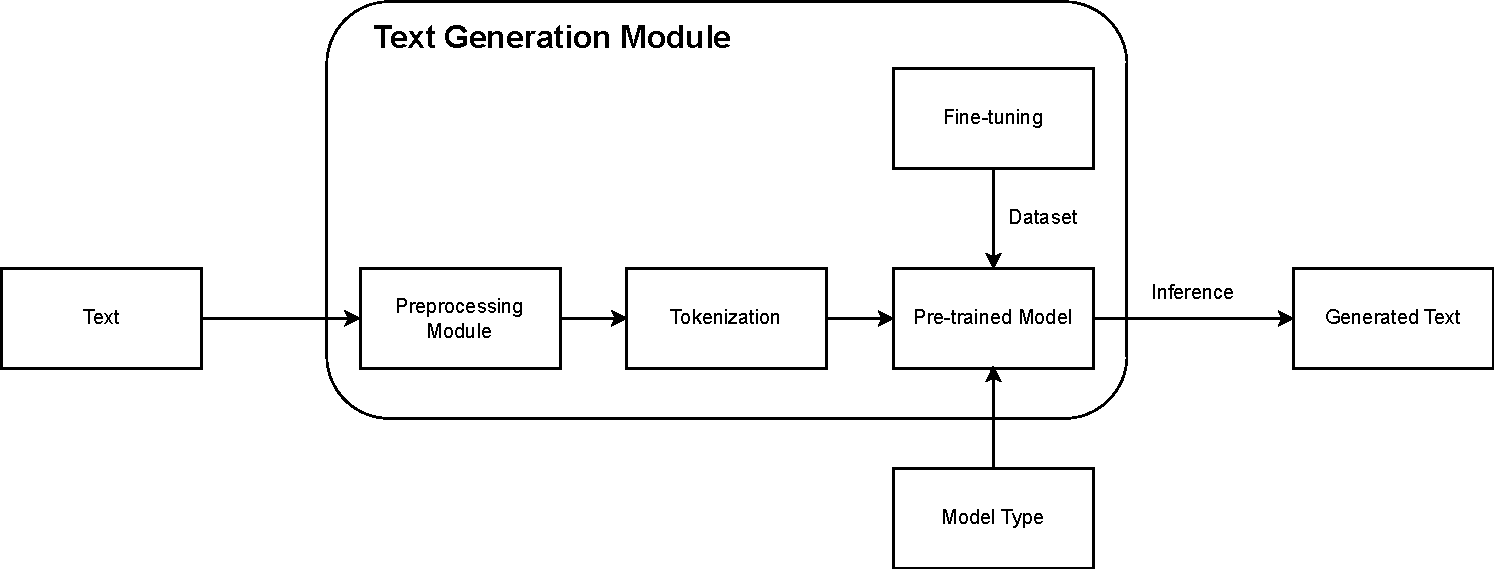
\includegraphics[width=\dimexpr\textwidth-2\fboxsep-2\fboxrule\relax,height=\dimexpr\textheight-2\fboxsep-2\fboxrule\relax,keepaspectratio,page=1]{diagram_1.pdf}}
\label{fig:design1}
\end{figure}

\begin{figure}[ht]
\centering
\caption{Flowchart depicting the process of generating a summary using TST}
\setlength{\fboxsep}{10pt}
%\setlength{\fboxrule}{1pt}
\fbox{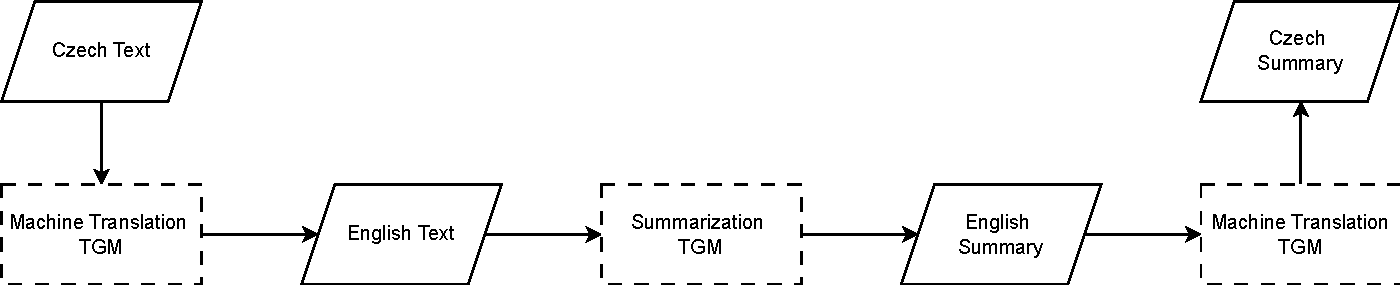
\includegraphics[width=\dimexpr\textwidth-2\fboxsep-2\fboxrule\relax,height=\dimexpr\textheight-2\fboxsep-2\fboxrule\relax,keepaspectratio,page=1]{diagram_2.pdf}}
\label{fig:design2}
\end{figure}

\section{Hugging Face} \label{hf}
%todo show some examples of CODE
Hugging Face\footnote{\url{https://huggingface.co/}} is a prominent platform in the machine learning community, providing an ecosystem for working with SOTA models and datasets. The platform hosts a vast collection of pre-trained models for various NLP tasks. One of the key contributions towards the platform's popularity is the Hugging Face Transformers~\cite{wolf-etal-2020-transformers} library, which provides a high-level abstraction for the usage of many large language models (LLM). It allows the users to perform inference, pre-training, and fine-tuning without a deep knowledge of the used architecture. 
 %Pre-training is the initial training of a model  on a large dataset, where the model gains general knowledge of the task or tasks it is trained on. Fine-tuning is the process of additional training of a pre-trained model for the purpose of improving the model's performance on specific tasks. 
%For an pre-training and fine-tuning example, T5 (described in Chapter \ref{methods}) is a model that was pre-trained on a variety of NLP tasks. However, it can be fine-tuned on a narrower or more specific dataset to enhance its performance for particular tasks such as text summarization, question answering, or translation. This fine-tuning process adapts T5 to the specific characteristics of the task at hand, leveraging the general knowledge it acquired during pre-training and applying it to solve the targeted problems more effectively.
\subsection{Hugging Face Transformers}
The Hugging Face Transformers (HFT)~\cite{wolf-etal-2020-transformers} library is a framework that supports the usage of thousands of pre-trained models for various machine learning tasks such as text, vision, and audio processing. It supports integration with popular machine learning libraries: PyTorch\footnote{\url{https://pytorch.org/}}, TensorFlow\footnote{\url{https://www.tensorflow.org/}}, and JAX\footnote{\url{https://jax.readthedocs.io/en/latest/}}.

The library offers not only high-level APIs for training and inference but also low-level access for more detailed customization.

The library also simplifies the deployment and usage of many models. For example, deploying a fine-tuned LongT5 for text generation can be done with just a few lines of code (see \ref{hf:pipeline_example}).

\subsubsection{Trainer} \label{hf:trainer}
For model training, we used HFT Trainer class\footnote{\url{https://huggingface.co/docs/transformers/main_classes/trainer}}. HFT Trainer allows users to train their models for specific tasks such as, but not limited to NLP, computer vision (object detection, image classification) or speech recognition.
The class provides an abstraction for the training loop, automating processes such as the forward and backward passes.

For dealing with computationally heavy tasks, it also supports distributed training across multiple GPUs, CPU offloading and disk offloading. The Trainer also supports \term{Parameter-Efficient Fine-Tuning} (PEFT)~\cite{peft} methods which significantly reduces hardware requirements for model training by fine-tuning only a fraction of the model's parameters rather than all of the model's parameters.
It also includes logging and monitoring functionalities, enabling users to track training metrics, such as training loss, validation loss, and evaluation metric scores on chosen metrics, throughout the training process.

\subsubsection{Inference} \label{impl:hf:inference}
Inference is the process of using a trained model to make predictions or decisions.
This process in text generation models, including those like mT5 and Mistral 7B, involves generating new text based on an input sequence of tokens. These models produce a probability distribution for each subsequent token, from which the next token is selected. The method of selection relies heavily on this probability distribution and the chosen text generation strategy for selecting subsequent tokens.

\paragraph{Settings}\label{impl:hf:inference_settings}
In HFT, several parameters can be adjusted to influence the text generation strategy, therefore affecting the model's output. These parameters include:
\begin{itemize}
    \item \texttt{max\_new\_tokens:} Max amount of tokens that can be generated.
    \item \texttt{do\_sample:} If set to \texttt{false}, uses default decoding strategy greedy search, where the token with the highest probability is always chosen. If set to \texttt{true}, allows the usage of different decoding strategies as described in Hugging Face documentation\footnote{\url{https://huggingface.co/docs/transformers/generation_strategies}}.
    \item \texttt{temperature:} Modifies the probability distribution of tokens. A higher temperature usually leads to a more uniform probability distribution.
    \item \texttt{top\_p:} Only tokens that cumulatively comprise up to \texttt{top\_p} probability can be chosen.
    \item \texttt{repetition\_penalty:} Penalizes previously generated tokens to reduce repetition in the output. For more details see \cite{keskar2019ctrl}.
\end{itemize}
Adjusting these parameters allows for modification of the generation process, allowing the creation of outputs that range from highly deterministic to varied and non-deterministic, depending on the desired outcome.

\paragraph{Pipeline} \label{hf:pipeline}
HFT also includes a feature known as the pipeline\footnote{\url{https://huggingface.co/docs/transformers/main_classes/pipelines}}. The pipeline simplifies the usage of inference without requiring extensive coding. A pipeline bundles together a model and its associated tokenizer, streamlining the workflow for common tasks such as text classification, named entity recognition, text generation, summarization, and more. Users can create a pipeline for the desired task using the \texttt{text} parameter and apply it to the input text. For a pipeline usage example in code, see \ref{hf:pipeline_example}.

%\lstset{style=FASThesisLstStyle,} %backgroundcolor=\color{fascolor!10}}

\begin{pythoncode}[language=Python, caption={Text summarization inference example using pipeline\label{hf:pipeline_example}}] 
from transformers import pipeline

text = "A long string for summarization." #text to be summarized
summarizer = pipeline(
    text = "summarization", #the performed task 
    model = "pszemraj/long-t5-tglobal-xl-16384-book-summary", #the model used
)
result = summarizer(text)
print(result[0]['summary_text']) #prints out summary to the console
\end{pythoncode}

\subsection{Hugging Face Datasets library}
Hugging Face Datasets\footnote{\url{https://huggingface.co/docs/datasets/index}} is a library for managing and creating datasets. Users can use the datasets library to load a variety of formatted datasets from the Hugging Face platform or they can load their own custom datasets through methods available in the library. By leveraging the Apache Arrow\footnote{\url{https://arrow.apache.org}} format, the library is optimized to process large datasets with high speeds and efficiency.

The SumeCzech dataset is only available through scripts provided by the author. However, the Hugging Face Datasets library supports many formats, including the JSON Lines format, which is the format that the SumeCzech dataset uses. 

\section{Creating Dataset for Model Evaluation} \label{impl:dataset}
We obtained data from Porta fontium~\cite{statni-oblastni-archiv-v-plzni-no-date}, more specifically, OCR-processed versions of historical journals, \textit{Posel od Čerchova} and \textit{Domažlické listy}. The received journals span a publication period from the 19th century up to the beginning of the 20th century. While constructing the dataset, we only used the texts from the journal \textit{Posel od Čerchova}.

Porta fontium~\cite{statni-oblastni-archiv-v-plzni-no-date} is a joint Czech-Bavarian project aimed at reconnecting historically significant archival materials related to Czech and German histories, which were physically separated in the past. Through digitization, this project facilitates the creation of a virtual collection, making these archives accessible to the public, researchers, and regional historians via a shared online platform.
\subsection{Dataset Format}
Before we started with the creation of the dataset, we had to decide on its format.
The dataset is therefore systematically organized, initially sorted by journal titles and their respective publication years. These journals are further divided into monthly issues, which are then subdivided into individual pages. A total summary of the issue resides alongside the list of individual pages. The structure of an individual page is as follows:
\begin{itemize}
    \item \textbf{text:} OCR-processed text extracted from the given page, a digital rendition of the original printed content.
    \item \textbf{summary:} Summary of the page, which is no more than 5 sentences long.
    \item \textbf{year:} Publication year of the journal.
    \item \textbf{journal:} This identifier specifies the issue source: the day, month, and the number of the issue is contained within this identifier.
    \item \textbf{page\_src:} The name of the file, where the contents of \textit{text} identifier come from.
    \item \textbf{page\_num:} The number of the page.
\end{itemize}
Initially, our approach was focused solely on summarizing individual pages. However, after consultations with the data providers at Porta fontium, we expanded our format to include a total summary for each issue in addition to the page summaries. For an example of the dataset's format, see \ref{impl:dataset:dataset_format}. 
\begin{code}{}{Showcase of the dataset format\label{impl:dataset:dataset_format}}
{
  "posel-od-cerchova-1882": {
    "03-30-n1": {
      "pages": [
        {
          "text": "Text from file described by page_src",
          "summary": "Summary of contents of text",
          "year": "1882",
          "issue": "03-30-n1",
          "page_src": "posel-od-cerchova-1872-03-30-n1_0010.jp2.txt",
          "page_num": 1
        }
      ],
      "summary_total": "Summary of issue 03-30-n1"
    }
  }
}
\end{code}
\subsection{Building the Dataset}
The construction of the dataset involved addressing the challenge of creating summaries for the provided texts, which were composed in historical Czech and in some rare cases even German. The texts also covered a variety of different topics, from local news surrounding Domažlice, opinion pieces, and various local advertisements to internal and worldwide politics and feuilletons. Furthermore, it was important to construct a dataset of sufficient size to ensure the accuracy and reliability of our evaluations. These aspects added complexity to the summarization task.

To overcome this, we employed SOTA LLMs, including GPT-4~\cite{openai2024gpt4} (specifically the \texttt{gpt-4-1106-preview} version) and Claude 3 Opus~\cite{anthropic-2024} (Opus) (specifically the \texttt{claude-3-opus-20240229} version), for text summary creation. These models were selected based on their SOTA performance in many NLP tasks. In regards to complete issue summaries, even though both models were capable of processing the entire issue all at once, we concatenated the summaries of the individual pages in their respective order and then summarized the concatenation. This approach was adopted because initial experiments revealed that summarizing the entire issue all at once led to overly broad summaries, due to the diverse range of topics covered within each issue. In contrast, summarizing concatenated individual page summaries preserved a higher level of detail.

While generating the summaries, it was crucial for them to be concise and due to the fact, that most implemented methods used the SumeCzech dataset for fine-tuning, we wanted the summaries to be created in the style of a news reporter. Therefore, all inputs to the models generating the summary were prepended with:
\lstset{style=plainsrc, numbers=none, breaklines=true, 	breakatwhitespace=True,}
\begin{lstlisting}
Vytvoř shrnutí následujícího textu ve stylu novináře. Počet vět <= 5:
\end{lstlisting}
Through this methodology, we summarized 432 pages, effectively resulting in the creation of 100 issue summaries. To ensure accuracy and prevention of any mistakes, the summaries underwent a human review. 

In our experience, we observed that while both models produced summaries of acceptable quality, Opus tended to create more succinct and stylistically appropriate summaries, closely aligning with the news reporter format. However, there were instances where summaries generated by Opus exhibited an excessive focus on a single topic. On the other hand, GPT-4 aimed to incorporate a greater level of detail within the five-sentence constraint but occasionally deviated from the specified stylistic prompt. 
When the model-generated summary exhibited significant stylistic deviations or excessive focus on a single topic, we either modified or regenerated it until an acceptable version was achieved.

\section{Summarization Models}
\subsection{mT5} \label{impl:mt5}
The decision to train the mT5 model was motivated by its multilingual capabilities and its proven track record in achieving success\footnote{\url{https://huggingface.co/csebuetnlp/mT5_multilingual_XLSum}}\footnote{\url{https://huggingface.co/tsmatz/mt5_summarize_japanese}} across various text summarization tasks in different languages. Despite the model being available in several sizes, constraints related to computational resources limited our efforts to the base variant, the only model size we managed to train successfully. 

The analysis of text and abstract word counts within the SumeCzech dataset is detailed in Table \ref{tab:text_word_count_metrics}. This analysis highlights the average, median, maximum, and minimum word counts across the different splits. Table \ref{tab:tokenized_text_abstract_metrics} presents a detailed analysis of the SumeCzech dataset after tokenization using the mT5 tokenizer. The table provides an analysis of token counts for the text and abstract across the training, development (validation), and test splits of the dataset, detailing average, median, maximum, and minimum values. In comparison with Table \ref{tab:text_word_count_metrics}, we can see that on average one word is approximately equivalent to two tokens. The model maximum context length is 512 tokens, therefore truncation of the text in the dataset was unavoidable.

\begin{table}[htbp]
    \centering
    \caption{Analysis of the SumeCzech text and abstract word count}
    \label{tab:text_word_count_metrics}
    \begin{tabular}{lcccc}
        \toprule
        \textbf{Metric} & {\textbf{Train}} & {\textbf{Dev}} & {\textbf{Test}} \\
        \midrule
        Text Average & 409 & 411 & 415 \\
        Text Median & 325 & 326 & 329 \\
        Text Maximum & 14 745 & 13 283 & 12 007 \\
        Text Minimum & 93 & 99 & 99 \\
        \midrule
        Abstract Average & 38 & 38 & 39 \\
        Abstract Median & 38 & 38 & 38 \\
        Abstract Maximum & 470 & 253 & 220 \\
        Abstract Minimum & 10 & 10 & 10 \\
        \bottomrule
    \end{tabular}
\end{table}

\begin{table}[htbp]
    \centering
    \caption{SumeCzech text and abstract analysis using mT5 tokenizer}
    \label{tab:tokenized_text_abstract_metrics}
    \begin{tabular}{lcccc}
        \toprule
        \textbf{Metric} & {\textbf{Train}} & {\textbf{Dev}} & {\textbf{Test}} \\
        \midrule
        \multicolumn{4}{l}{\textbf{Text Token Count}} \\
        \midrule
        Average & 902 & 907 & 917 \\
        Median & 719 & 720 & 731 \\
        Maximum & 32 857 & 28 744 & 26 473 \\
        Minimum & 185 & 196 & 193 \\
        \midrule
        \multicolumn{4}{l}{\textbf{Abstract Token Count}} \\
        \midrule
        Average & 85 & 85 & 86 \\
        Median & 85 & 85 & 86 \\
        Maximum & 885 & 540 & 459 \\
        Minimum & 13 & 15 & 15 \\
        \bottomrule
    \end{tabular}
\end{table}




\subsubsection{Training}
The base variant of the mT5, which is a 580 million parameter model, was used for fine-tuning on SumeCzech dataset. Training was done using HFT Trainer. No optimization techniques such as PEFT (as discussed in Section \ref{hf:trainer}) were used. Each article text and abstract were first tokenized using the mT5 tokenizer and then truncated to 512 tokens.

The optimizer used was AdamW, the learning rate was set to 0.001 (as used by authors of mT5~\cite{xue-etal-2021-mt5} in their own fine-tuning experiments), weight decay was set to 0.01, and batch size was set to 8. Initial attempts at bigger batch sizes or longer sequences led to out of memory (OOM) errors. The training was conducted over 8 epochs, totalling 867500 steps, on a single NVIDIA A40 GPU. The training duration was 168 hours. Additionally, a linear scheduler was employed to adjust the learning rate over time.
\paragraph{Further Training}
Unlike Mistral 7B in Section \ref{impl:m7b}, we deemed further training on the dataset created for evaluation as fruitless due to the 512 token maximum context length available on mT5 being far exceeded by the amount of tokens in each of the pages of the dataset.
\subsection{Mistral 7B} \label{impl:m7b}
The task of fine-tuning an LLM requires significant computational resources. The fine-tuning of the base variant of mT5 with only 580M parameters led to near full capacity usage of the 45 GB VRAM available in the NVIDIA A40 GPU. In the case of Mistral 7B, a normal fine-tuning would be impossible on the given GPU. To train such a large model, we had to either reserve more GPUs or use various optimizations. Due to time constraints that came with reserving more GPUs from MetaCentrum\footnote{\url{https://metavo.metacentrum.cz/}} facilities, we opted to use the latter option.
\subsubsection{Optimization}
The optimization methods or libraries that were used during fine-tuning of Mistral 7B are briefly described in this section.
\paragraph{Unsloth}\label{impl:unsloth}
Unsloth~\cite{unsloth} is a library that is designed to make fine-tuning LLMs faster and more memory efficient. This is achieved through various optimizations like manual derivation of backpropagation steps and the use of OpenAI's Triton\footnote{\url{https://github.com/openai/triton}} language for kernel rewriting. Developed by Daniel Han, Michael Han, and the open-source community, it is fully compatible with the Hugging Face ecosystem which includes the Hugging Face Transformer library, therefore usage with HFT Trainer is possible. As of this writing, the amount of supported architectures is limited. From the models described in Chapter \ref{methods}, only Mistral architecture models are supported. Fine-tuning with multiple GPUs is currently not supported.
\paragraph{Quantization}
\term{Quantization}~\cite{jacob2017quantization} is a technique used to reduce the computational cost and model size of neural networks by approximating the weights and activations with lower bit representations. Common quantizations are \texttt{float32} to \texttt{float16} and \texttt{float32} to \texttt{int8} (8-bit integer). There are various types of quantization methods~\cite{gholami2021survey} such as \term{Post-Training Quantization} (PTQ) or \term{Quantization-Aware Training} (QAT). 

PTQ calibrates the model first and then it applies quantization to the model. The model is calibrated using a subset of the training data to determine the optimal way to map floating-point numbers to a lower-bit representation. However, PTQ might lead to a larger drop in accuracy when compared to QAT.

With QAT the model is quantized and then fine-tuned using a subset of the training data. The weights are then updated in a way that the model learns how to perform well even with quantized values. QAT has usually higher accuracy than PTQ but requires more time due to fine-tuning.
\paragraph{Low-Rank Adaptation}\label{impl:lora}
\term{Low-Rank Adaptation} (LoRA)~\cite{hu2021lora} is a method to adapt large LLMs to specific tasks (such as text summarization) in a more parameter-efficient way. The key idea behind LoRA is to freeze the pre-trained model weights and introduce trainable low-rank matrices that modify the behavior of the model. LoRA works by injecting these low-rank matrices into specific layers of the Transformer architecture. The layers are selected based on several factors, such as the downstream task or model's architecture. The matrices then alter the output of the layers which they are injected into. This results in a much lower memory requirement and a reduction in the computational resources needed for adaptation in comparison to full fine-tuning, where all parameters are adjusted, while achieving similar performance.
\paragraph{QLoRA}
\term{QLoRA}~\cite{dettmers2023qlora} is a fine-tuning method that significantly reduces the memory needed to fine-tune large language models by combining quantization and LoRA together. It first quantizes the pre-trained language model to 4-bit using a novel method. Then it introduces LoRA into the quantized model. During fine-tuning, the backpropagation only tunes the low-rank matrices. QLoRA uses bitsandbytes\footnote{\url{https://github.com/TimDettmers/bitsandbytes}} for quantization and it is fully supported by the Hugging Face Transformers library as a PEFT method.

\subsubsection{Training}
We encountered some problems during the initial installation and usage of the Unsloth library. The library uses \command"ldconfig"\footnote{\url{https://man7.org/linux/man-pages/man8/ldconfig.8.html}} command to create the necessary links for the CUDA library. However, this command accesses and writes into the \texttt{/etc/} directory which requires root permissions. The environment in which the training was done does not grant root permissions by default. To avoid using root permissions, we set the environment variable \texttt{TRITON\_LIBCUDA\_PATH} to \filename{/usr/local/cuda/compat}, which is a directory where \filename{libcuda.so} file resided. We also set the environment variable \texttt{LIBRARY\_PATH} to \filename{/usr/local/cuda/lib64}, which in our case is a path where libraries necessary for the development and execution of CUDA applications are located.

To fine-tune Mistral 7B, we utilized resources from publicly available fine-tuning notebooks\footnote{\url{https://jupyter.org/}}\footnote{\url{https://colab.google/}} and a 4-bit pre-quantized Mistral 7B model\footnote{\url{https://huggingface.co/unsloth/mistral-7b-bnb-4bit}} from Hugging Face platform, both provided by the developers of Unsloth library. In contrast to the utilization of HFT Trainer for the mT5 model fine-tuning, we use SFTTrainer\footnote{\url{https://huggingface.co/docs/trl/sft_trainer}} from TRL~\cite{vonwerra2022trl} library, which serves as a wrapper for HFT Trainer.

The model was fine-tuned on the SumeCzech dataset for one epoch with a total batch size of 32, therefore the training took 27112 steps in total. The whole process took 400 hours and the model was fine-tuned using 1x NVIDIA A40 45GB. Initially, a broader training scope beyond one epoch was considered. However, such training would have required more time than was available for this thesis.
\paragraph{Dataset Processing}
To pass the SumeCzech dataset into the SFTTrainer, we needed to format the dataset first. We formatted the dataset using the format used in the Stanford Alpaca project \cite{alpaca}\cite{touvron2023llama}\cite{wang2023selfinstruct}. Each dataset entry had these columns after formatting:
\begin{itemize}
  \item \textbf{input:} The full text of the article.
  \item \textbf{output:} The summary of the article.
  \item \textbf{instruction:} The instruction for the model. The instruction was set to \mytexttt{Summarize the following text:} for all entries.
  \item \textbf{text:} The combination of input, output, and instruction in a structured format. See \ref{impl:mistral:dataset_format} for an example. Each text had to be appended with an end-of-sequence (EOS) token \texttt{<s>}.
\end{itemize}
\lstset{style=FASThesisLstStyle,} %backgroundcolor=\color{fascolor!10}}
\begin{lstlisting}[caption={Example of \texttt{text} column in formatted SumeCzech dataset entry. The input and response were truncated and appended with \texttt{...} due to their long length\label{impl:mistral:dataset_format}}] 
Below is an instruction that describes a task, paired with an input that provides further context. Write a response that appropriately completes the request.

### Instruction:
Summarize the following text:

### Input:
Kdy jste slyšela jako cizinka slovo Ostrava poprvé? O Ostravě jsem poprvé slyšela v Českých Budějovicích, byla jsem tam asi rok v angažmá...

### Response:
Pračiková žije v Ostravě už téměř dvacet let... <s>
\end{lstlisting}

\paragraph{Parameters}
The training utilizes \term{Mixed Precision Training}~\cite{micikevicius2018mixed} method, where some variables are stored at half-precision (\texttt{float16} or \texttt{Bfloat16}~\cite{kalamkar2019study} instead of the standard full-precision \texttt{float32}). This does make computations faster, although it does not reduce the memory requirements. We specifically use \texttt{Bfloat16}. The max sequence length was set to 8192. The batch size was set to 8 with gradient accumulation steps set to 4, which makes an effective batch size of 32. Learning rate was set to $2 \times 10^{-4}$, which was the value used by the authors of Unsloth library in their own fine-tuning notebooks. The optimizer used was 8-bit AdamW with 0.01 weight decay along with a linear learning rate scheduler. For \term{QLoRA} parameters, we used rank at 16 and alpha at 16. The targeted layers were \texttt{q\_proj}, \texttt{k\_proj}, \texttt{v\_proj}, \texttt{o\_proj}, \texttt{gate\_proj}, \texttt{up\_proj} and \texttt{down\_proj}. Warmup steps were set to 100.

\subsubsection{Further Training} \label{impl:mistral:furthertraining}
After the initial training on the SumeCzech dataset was complete, we employed further training on the model using the dataset described in Section \ref{impl:dataset} due to unsatisfactory performance. We further elaborate on the performance in Chapter \ref{ch:eval}.

The evaluation dataset was divided into a non-shuffled 75-25 ratio for the train and test splits, yielding 324 page summaries for the training set and 108 for the testing set. Subsequently, the model underwent an additional 16 epochs of training on the training split.

A validation set was not constructed for several reasons. Initially, an issue was encountered where the validation loss consistently returned a Not a Number (NaN) value. This issue had also appeared during the initial training phase; however, it was deemed less critical then due to the one epoch training duration, which minimized the risk of overfitting~\cite{komatsuzaki2019epoch}. Furthermore, given the constrained size of our dataset, it was important to maintain a test set of adequate size to ensure the quality of the evaluation. 

The absence of validation loss meant we lacked a method to identify overfitting. To overcome this, we implemented a strategy of saving checkpoints after each training epoch. We then assessed the performance of these checkpoints on the test set using ROUGE\textsubscript{RAW} metrics, selecting the epoch that demonstrated the best performance. Details of this process are further discussed in Chapter \ref{ch:eval}.

Total summaries were not utilized in this phase of training due to the complete issue text length exceeding the model maximum context length capacity.
\paragraph{Parameters}
The training parameters were largely maintained as they were during the initial phase, with a few modifications: the batch size was adjusted to 8, and gradient accumulation steps were set at 1, effectively setting the batch size at 8. Warmup steps were calculated as 10\% of the total training steps; with 16 epochs leading to a total of 640 steps, this resulted in 64 warmup steps.

\section{TST}
We implemented the TST method as stated in the method study described in Chapter \ref{methods}, Section \ref{methods:translate}. For high-quality translation, the ALMA-R 13B variant was utilized, while English text summarization was performed using the 4-bit pre-quantized, instruct fine-tuned variant of Mistral 7B\footnote{\url{https://huggingface.co/unsloth/mistral-7b-instruct-v0.2-bnb-4bit}}, made available by the Unsloth library developers on the Hugging Face platform. The ALMA-R 13B model, in its non-quantized form, was downloaded and subsequently quantized using the bitsandbytes\footnote{\url{https://github.com/TimDettmers/bitsandbytes}} library.

During the translation, we encountered challenges associated with the ALMA-R 13B model. Specifically, the model's maximum context length of 4096 tokens and a noticeable drop in translation quality for long texts were the biggest concerns. This decline in performance can be attributed to the model being fine-tuned on input texts with a maximum of 512 tokens, as detailed in \cite{xu2024contrastive}. To prevent this, texts were divided into segments of 10 sentences each for translation. These segments were then translated independently and reassembled to produce the complete translation. 

The translation quality however varied with the number of sentences per segment, which in turn affected the quality of subsequent summarization. Specifically, larger segments sometimes resulted in the model's outputs repeating its generated sequences, while smaller ones, though less repetitive, provided insufficient context which negatively affected the translation quality. We achieved best results with 10-sentence segments, using inference settings of \texttt{temperature} and \texttt{top\_p} set to 1, and \texttt{repetition\_penalty} set to 1.3.

For summarization, a specific template supported by the model tokenizer was used, as shown in an example \ref{impl:tst:mistralprompt}.

\lstset{style=FASThesisLstStyle,} %backgroundcolor=\color{fascolor!10}}
\begin{lstlisting}[caption={Summarization template for TST\label{impl:tst:mistralprompt}}] 
[{
        "role": "user",
        "content": "Summarize my texts using only 5 sentences"
    },
    {
        "role": "assistant",
        "content": "Sure. I will write summaries in the style of a news reporter and use only 5 sentences."
    },
    {
        "role": "user",
        "content": "The text to summarize..."
}]    
\end{lstlisting}
The template shown in \ref{impl:tst:mistralprompt} was processed using the tokenizer \mytexttt{apply\_chat\_template} function, which converts the list into a formatted string prompt. This prompt was immediately tokenized because the parameter \texttt{tokenize} is to \texttt{true} by default. This specific template was used because the model had problems with following instructions, usually generating more than 5 sentences or summarizing text in different styles. The inference settings were also adjusted to a \texttt{temperature} of 0.3 and \texttt{top\_p} to 1 for higher adherence to instructions. The model also had a tendency to enumerate sentences, therefore regular expressions were used to remove them. The process for translating the English summaries back to Czech language followed the same procedure as the initial translation process with the languages swapped.

\chapter{Evaluation}\label{ch:eval}
This chapter focuses on evaluating the methods implemented, as detailed in Chapter \ref{char:implementation}. We will assess the performance of both mT5 and Mistral 7B, which were trained on the SumeCzech dataset. Moreover, these models will be evaluated on the SumeCzech test set to gain a comprehensive understanding of their capabilities. Evaluation will be conducted on a dataset created in Chapter \ref{char:implementation}, hereafter referred to as the POC (Posel od Čerchova) dataset for conciseness. The POC dataset comprises of two types of summaries: issue summaries (POC-I) and page summaries (POC-P). Additionally, we will outline the evaluation settings employed. If specific inference settings were not mentioned, it implies that the default settings were utilized. These defaults are detailed in the Hugging Face documentation\footnote{\url{https://huggingface.co/docs/transformers/main_classes/text_generation\#transformers.GenerationConfig}}. All evaluations in this Chapter will be done using the ROUGE\textsubscript{RAW} metric.

For ease of reference, we will be using various abbreviations. A list of these abbreviations is provided in Table \ref{tab:abbreviations}.

In the upcoming sections, we will compare the performance of these models. In the comparison tables, a value highlighted in \textbf{bold} will denote the highest value obtained.

\begin{table}[ht]
    \centering
    \caption{List of abbreviations}
    \label{tab:abbreviations}
        \begin{tabular}{ll}
        \hline
        \textbf{Abbreviation} & \textbf{Description}                                             \\ \hline
        POC                   & Posel od Čerchova dataset                                        \\
        POC-I                 & Issue summaries from the POC dataset                             \\
        POC-P                 & Page summaries from the POC dataset                              \\
        M7B-SC                & Mistral 7B model trained on the SumeCzech dataset                 \\
        M7B-POC               & M7B-SC further trained on the POC dataset               \\
        mT5-SC                & mT5 model trained on the SumeCzech dataset                        \\
        TST                   & Translate-Summarize-Translate method                           \\ \hline
    \end{tabular}
\end{table}
 

\section{Performance of SumeCzech Trained Models on SumeCzech Test Set}
This section examines the results of the mT5-SC and M7B-SC models on the SumeCzech dataset. The results can be seen in Table \ref{tab:eval:sc_scores_comparison}. Additionally, this evaluation includes comparative analyses with methodologies utilized by the creators of SumeCzech and a fine-tuned mBART model, referred to as HT2A-S. The HT2A-S model, developed by Marian Krotil in their Bachelor's thesis~\cite{Krotil2022TextSummarization}, was trained using a slightly different methodology; the article headline was included with the text during abstract generation. However, the author also included an evaluation of HT2A-S on text-to-abstract generation excluding the headline incorporation, which is the evaluation presented in Table \ref{tab:eval:sc_scores_comparison}. 

Extractive methods, evaluated by SumeCzech authors, like Textrank (see \ref{textrank}), and simplistic strategies such as selecting the first few sentences or random sentences for summaries, are also compared. An abstractive text summarization model developed using the tensor2tensor~\cite{tensor2tensor} framework by the SumeCzech authors is evaluated as well. Among all the various methods, M7B-SC demonstrates superior performance across all listed evaluation metrics.

\begin{table}[ht]
    \centering
    \caption{Results of various methods on SumeCzech test set}
    \label{tab:eval:sc_scores_comparison}
    \begin{tabular}{
        l
        S
        S
        S
        S
        S
        S
        S
        S
        S
    }
        \toprule
        Method & \multicolumn{3}{c}{ROUGE\textsubscript{raw}-1} & \multicolumn{3}{c}{ROUGE\textsubscript{raw}-2} & \multicolumn{3}{c}{ROUGE\textsubscript{raw}-L} \\
        \cmidrule(lr){2-4} \cmidrule(lr){5-7} \cmidrule(lr){8-10}
        & {P} & {R} & {F} & {P} & {R} & {F} & {P} & {R} & {F} \\
        \midrule
        M7B-SC & \textbf{24.4} & \textbf{19.7} & \textbf{21.2} & \textbf{6.5} & \textbf{5.3} & \textbf{5.7} & \textbf{17.8} & \textbf{14.5} & \textbf{15.5} \\
        mT5-SC & 22.0 & 17.9 & 19.2 & 5.3 & 4.3 & 4.6 & 16.1 & 13.2 & 14.1 \\
        \midrule
        HT2A-S & 22.9 & 16.0 & 18.2 & 5.7 & 4.0 & 4.6 & 16.9 & 11.9 & 13.5 \\
        first & 13.1 & 17.9 & 14.4 & 0.1 & 9.8 & 0.2 & 1.1 & 8.8 & 0.9 \\
        random & 11.7 & 15.5 & 12.7 & 0.1 & 2.0 & 0.1 & 0.7 & 10.3 & 0.8 \\
        textrank & 11.1 & 20.8 & 13.8 & 0.1 & 6.0 & 0.3 & 0.7 & 13.4 & 0.8 \\
        tensor2tensor & 13.2 & 10.5 & 11.3 & 0.1 & 2.0 & 0.1 & 0.2 & 8.1 & 0.8 \\
        \bottomrule
    \end{tabular}
\end{table}
\section{Evaluating M7B-SC and M7B-POC on the POC-P Test Set}
As discussed in Chapter \ref{char:implementation}, specifically in Section \ref{impl:mistral:furthertraining}, the performance of M7B-SC on the POC-P dataset was deemed unsatisfactory. To address this, we conducted further training and monitored the model's progress by saving a checkpoint at the end of each epoch, yielding a total of 16 checkpoints. These checkpoints allowed us to evaluate the model performance on the POC-P test set at each epoch, with the results presented in Table \ref{tab:eval:checkpoints_scores}.

Our analysis revealed that M7B-SC performance on the POC-P test set was significantly lower than M7B-POC performance from the very first epoch of further training. Notably, the model demonstrated its highest overall performance at the third epoch. Based on this finding, we selected the third epoch checkpoint to represent the M7B-POC model for subsequent evaluations and comparisons.

\begin{table}[ht]
    \centering
    \captionsetup{font=scriptsize}
    \caption{Comparison of M7B-POC's performance at various epochs on POC-P test set. Epoch 0 represents the performance of the M7B-SC model.}
    \label{tab:eval:checkpoints_scores}
    \begin{tabular}{
        l
        S
        S
        S
        S
        S
        S
        S
        S
        S
    }
        \toprule
        Epoch & \multicolumn{3}{c}{ROUGE\textsubscript{raw}-1} & \multicolumn{3}{c}{ROUGE\textsubscript{raw}-2} & \multicolumn{3}{c}{ROUGE\textsubscript{raw}-L} \\
        \cmidrule(lr){2-4} \cmidrule(lr){5-7} \cmidrule(lr){8-10}
        & {P} & {R} & {F} & {P} & {R} & {F} & {P} & {R} & {F} \\
        \midrule
            0 & 19.9 & 5.1 & 7.1 & 2.9 & 0.8 & 1.1 & 15.2 & 3.9 & 5.4 \\
        1 & 23.6 & 15.7 & 18.1 & 3.6 & 2.4 & 2.8 & \textbf{16.8} & 11.2 & 12.8 \\
        2 & \textbf{24.1} & 16.2 & 18.9 & 4.2 & 2.8 & 3.3 & 16.4 & 11.1 & 12.9 \\
        \midrule
        3 & 23.3 & 17.4 & 19.5 & \textbf{4.7} & \textbf{3.5} & \textbf{4.0} & 16.4 & 12.3 & \textbf{13.8} \\
        \midrule
        4 & 22.8 & 17.5 & 19.4 & 4.1 & 3.1 & 3.5 & 15.3 & 11.8 & 13.1 \\
        5 & 22.1 & 20.1 & \textbf{20.6} & 3.7 & 3.5 & 3.5 & 14.5 & 13.0 & 13.4 \\
        6 & 22.2 & 19.3 & 20.4 & 3.9 & 3.4 & 3.6 & 14.6 & 12.7 & 13.4 \\
        7 & 22.1 & 18.8 & 19.9 & 3.7 & 3.1 & 3.3 & 14.4 & 12.3 & 13.0 \\
        8 & 21.2 & \textbf{20.2} & 20.4 & 3.6 & 3.3 & 3.4 & 13.7 & \textbf{13.1} & 13.2 \\
        9 & 21.0 & 19.5 & 19.9 & 3.6 & 3.3 & 3.4 & 13.3 & 12.3 & 12.6 \\
        10 & 21.4 & 19.5 & 20.0 & 3.3 & 3.0 & 3.1 & 13.8 & 12.5 & 12.9 \\
        11 & 20.6 & 18.6 & 19.1 & 3.4 & 3.1 & 3.1 & 13.7 & 12.3 & 12.6 \\
        12 & 20.1 & 19.7 & 19.5 & 3.4 & 3.3 & 3.2 & 13.2 & 13.0 & 12.8 \\
        13 & 20.0 & 19.1 & 19.3 & 3.0 & 2.9 & 2.9 & 13.0 & 12.5 & 12.6 \\
        14 & 20.7 & 19.9 & 19.9 & 3.3 & 3.3 & 3.2 & 13.2 & 12.8 & 12.7 \\
        15 & 20.8 & 19.5 & 19.8 & 3.4 & 3.2 & 3.2 & 13.5 & 12.6 & 12.8 \\
        16 & 21.1 & 19.4 & 19.7 & 3.3 & 3.0 & 3.1 & 13.6 & 12.4 & 12.6 \\
        \bottomrule
    \end{tabular}
\end{table}


\section{Performance of Implemented Methods on POC-P and POC-I}\label{eval:res_poc}
The performance of M7B-POC, mT5, and TST can be seen in Table \ref{tab:eval:poc-p} for POC-P and Table \ref{tab:eval:poc-i} for POC-I. The asterisk (*) indicates that the model was evaluated on a subset of the POC-P test set, respectively the subset of the POC-I test set. Specifically, it was evaluated on 106 page summaries, respectively 25 issue summaries. Out of the original test set's 108 page summaries and 26 issue summaries, two page summaries and one issue were discarded because the two page summaries did not contain enough information to form a complete issue summary. TST and mT5-SC were evaluated on all page summaries in POC-P and all issue summaries in POC-I.

The analysis indicates that M7B-POC exhibits the best overall performance on both the POC-P and POC-I datasets. In contrast, the TST method achieved higher recall scores, likely due to generating longer summaries than M7B-POC, albeit with reduced precision. It's worth noting that M7B-POC's performance slightly varies from the results observed at the third epoch in \ref{tab:eval:checkpoints_scores}, attributed to the exclusion of the two page summaries from the evaluation.

During the generation of issue summaries, M7B-POC encountered a specific problem where it produced summaries that appeared to be mere concatenations of page summaries. To address this, we adjusted the inference settings by setting the \texttt{temperature} to 0.6, \texttt{top\_p} to 0.8, enabling \texttt{do\_sample} as \texttt{true}, and adjusting the \texttt{repetition\_penalty} to 1.1. These modifications resulted in the generation of more appropriate issue summaries, according to our observations.
\begin{table}[ht]
    \centering
    \captionsetup{font=scriptsize}
    \caption{Results of implemented methods on POC-P. See Section \ref{eval:res_poc} and Table \ref{tab:abbreviations} for more details.}
    \label{tab:eval:poc-p}
    \begin{tabular}{
        l
        S
        S
        S
        S
        S
        S
        S
        S
        S
    }
        \toprule
        Method & \multicolumn{3}{c}{ROUGE\textsubscript{raw}-1} & \multicolumn{3}{c}{ROUGE\textsubscript{raw}-2} & \multicolumn{3}{c}{ROUGE\textsubscript{raw}-L} \\
        \cmidrule(lr){2-4} \cmidrule(lr){5-7} \cmidrule(lr){8-10}
        & {P} & {R} & {F} & {P} & {R} & {F} & {P} & {R} & {F} \\
        \midrule
        M7B-POC* & \textbf{23.5} & 17.4 & 19.6 & \textbf{4.8} & 3.5 & \textbf{4.0} & \textbf{16.6} & 12.2 & \textbf{13.8} \\
        TST & 17.2 & \textbf{25.1} & \textbf{19.9} & 2.5 & \textbf{3.8} & 2.9 & 11.3 & \textbf{16.4} & 13.0 \\
        mT5-SC & 20.2 & 8.2 & 11.1 & 1.4 & 0.5 & 0.7 & 14.9 & 6.1 & 8.2 \\
        \bottomrule
    \end{tabular}
\end{table}

\begin{table}[ht]
    \centering
    \captionsetup{font=scriptsize}
    \caption{Results of implemented methods on POC-I. See Section \ref{eval:res_poc} and Table \ref{tab:abbreviations} for more details.}
    \label{tab:eval:poc-i}
    \begin{tabular}{
        l
        S
        S
        S
        S
        S
        S
        S
        S
        S
    }
        \toprule
        Method & \multicolumn{3}{c}{ROUGE\textsubscript{raw}-1} & \multicolumn{3}{c}{ROUGE\textsubscript{raw}-2} & \multicolumn{3}{c}{ROUGE\textsubscript{raw}-L} \\
        \cmidrule(lr){2-4} \cmidrule(lr){5-7} \cmidrule(lr){8-10}
        & {P} & {R} & {F} & {P} & {R} & {F} & {P} & {R} & {F} \\
        \midrule
        M7B-POC* & \textbf{19.3} & 17.6 & \textbf{18.0} & \textbf{3.2} & 2.8 & \textbf{2.9} & 13.7 & 12.4 & \textbf{12.8} \\
        TST & 14.0 & \textbf{24.8} & 17.5 & 1.7 & \textbf{3.1} & 2.1 & 9.1 & \textbf{16.3} & 11.4 \\
        mT5-SC & 18.2 & 5.9 & 8.6 & 1.0 & 0.3 & 0.4 & \textbf{14.0} & 4.5 & 6.5 \\
        \bottomrule
    \end{tabular}
\end{table}
\section{Examples and Discussion}
We present two examples of generated summaries. The first example, shown in Table \ref{eval:tab:example1}, includes page summaries from the 38th issue of Posel od Čerchova, 1882. The second example, in Table \ref{eval:tab:example2}, features issue summaries of the 52nd issue of the same publication from the same year.

The summaries in Table \ref{eval:tab:example1} generally convey similar information as the reference summary to a certain extent. However, the mT5-SC summary is just a composition of the first two sentences of the original text, which is not shown here due to its length. Both the M7B-POC and TST summaries contain grammatical errors. While the M7B-POC summary is slightly more coherent and better structured, it also includes more factual inaccuracies, as evident in its concluding sentence, where it mistakenly mentions the city of Prague as one of the donors and attributes the Weihburggasse street to the wrong village.

The following example in Table \ref{eval:tab:example2} shows comparable results. The mT5-SC summary was irrelevant. The M7B-POC summary has slightly better coherence and grammar in comparison to TST summary, however, it misinforms by not stating that the death of "sultánka" is a fictional event.

In our limited observations of these generated summaries and many other generated summaries, M7B-POC tended to create slightly more coherent summaries with better grammar, but TST produced less factual errors than M7B-POC.
\begin{table}[h!] 
\centering
\caption{Summaries of 'Posel od Čerchova,' page 5 of the 38th issue, 1882}
\label{eval:tab:example1}
\begin{tabular}{@{}p{0.95\textwidth}@{}} 
\toprule
\textbf{Reference} \\
\midrule
{\small V Petrohradě došlo k otravě osmi běloušů, kteří měli táhnout korunovační vůz cara Alexandra III. při jeho korunovaci v Moskvě. Koně byli nalezeni mrtví ve stáji carského paláce. Obce Milaveč a Radonice v okresu Domažlice přispěly na znovuzřízení Národního divadla, čímž mohou jít příkladem ostatnímu venkovu. Článek dále uvádí tržní ceny různých produktů v Domažlicích a Praze.} \\
\midrule
\textbf{M7B-POC} \\
{\small V Petrohradě byli otráveni osm carští bělouši, kteří měli táhnouti korunovační vozku pro cara Alexandra III. v Moskvě. V Domažlicích byly zaznamenány tržní ceny potravin a dalších zboží, včetně cen za talíře a sklenice. V Praze a Weihburggasse 26 v Milaveči a Radonicích I. byly oznámeny příspěvky na obnovu Národního divadla.} \\
\midrule
\textbf{TST} \\
{\small V Petrohradě byly v koníčkách palácových stájí nalezeny osm bílých koní, kteří zemřeli na otravu, určených pro korunovaci cara Alexandra III. V českém okrese Domažlice se loni dvě obce podílely na obnově Národního divadla a další mohou následovat jejich příklad. V následujícím textu jsou uvedeny ceny různých položek v Praze: Neffův obchod na Staroměstském náměstí za 39 J. Milaveč a Radonice I. v ulici Weihburggasse 26 vybraly za měsíc 10 zl. díky úsilí několika odvážných občanů.} \\
\midrule
\textbf{mT5-SC} \\
{\small Carští koně otráveni. Oněch osm běloušů, kteří měli korunní vůz při korunovací carovi Alexandra III. v Moskvě táhnouti, nalezli služebníci ve stáji paláce carského v Petrohradě zdatná ležeti Dla -x-1 byly snad jediné obce v okresu Domažlice.} \\
\bottomrule
\end{tabular}
\end{table}

\begin{table}[h!] 
\centering
\caption{Summaries of 'Posel od Čerchova,' 52nd issue, 1882}
\label{eval:tab:example2}
\begin{tabular}{@{}p{0.95\textwidth}@{}} 
\toprule
\textbf{Reference} \\
\midrule
{\small Domažlický týdeník "Posel od Čerchova" vstupuje do 11. ročníku svého vydávání s čtvrtletním předplatným variujícím dle způsobu doručení. V aktuálním vydání týdeník pokrývá široké spektrum témat, od politických událostí v Bosně, Tyrolsku, až po tragické incidenty v Srbsku a soudní případy v Paříži. Součástí obsahu je také pokračování povídky "Ze života sultánky", odhalení pomníku knížete Michajla v Bělehradě, a záměr francouzského ministra války rozšířit armádu. Zajímavostí jsou novinky na trhu, jako Hellerovy hrací stroje, a opatření pražské městské rady proti novoroční žebrotnické praxi mezi městskými zaměstnanci.} \\
\midrule
\textbf{M7B-POC} \\
{\small Posel od Čerchova informuje o politických událostech, jako jsou předlohy o výpomoci v Tyrolsku a Korutanech, rakousko-německém napětí a ruské vojenské aktivitě. Dále se diskutuje o stavebních pracích v Tyrolsku a Korutanech, financovaných zemskou zárukou. Zmíněna je nová předloha o založení samostatného církevního systému v Sarajevu, umožňující větší autonomii muslimské komunity. Dále je zmíněna popisná smrt sultánky ze Cařihradu, jejího vyhnanství po milostném vztahu s bratrem, a slavnostní odhalení pomníku knížeti Miloše Obrenoviče v Bělehradě. Dále jsou zmíněny kulturní události, jako je nová výstava uměleckých prací v Plzni, a společenské události, jako je nová výzva do sněmu v Bělehradě, a trestní události, jako jsou vraždy a zatčení v několika městech.} \\
\midrule
\textbf{TST} \\
{\small ČERCHOVSKÝ TÝDENÍK (POŠLA OD ČERCHOVA), noviny z Domažlic, pokrývají politická, obecná a komunitní témata v daném regionu. Ceny předplatného se liší. V Bosně byla založena náboženská organizace pro bosenskou muslimskou církev, zatímco ve městě Krivošiji byly z důvodu počasí pozastaveny stavební práce. V Srbsku zůstává Královský sněm krále Milana prázdný a situace je po volbách, jejichž cílem bylo nahradit radikální poslance, klidná. V Egyptě jsou odsouzení vůdci arabského povstání veřejně zesměšňováni a poté vysídleni, v České republice došlo k fatálnímu střetu mezi sousedy. Probíhají různé akce, například oslavy jmenování pana Justina V. Práška na funkci ředitele, jmenování paní Karol Fremuthové do funkce a hudební zkoušky pro taneční zábavy 26. prosince. Dále se zde koná loterie ve prospěch organizace „Matica“ a je zveřejněna kniha „Humory“. Společnost Singer nabízí originální šicí stroje jako ideální vánoční dárek.} \\
\midrule
\textbf{mT5-SC} \\
{\small Vánoční svátky jsou v plném proudu a s nimi i přípravy na vánoční svátky. Přinášíme vám plné znění projevu prezidenta republiky Václava Klause, který přednesl ve Vladislavském sále Pražského hradu.} \\
\bottomrule
\end{tabular}
\end{table}
\chapter{Conclusion}
In this Bachelor thesis, we introduced three methods which can summarize historical documents: mT5-SC, M7B-POC and TST with mT5-SC, M7B-SC and M7B-POC available on the Hugging Face platform\footnote{\url{https://huggingface.co/tranv/mt5-base-finetuned-sumeczech}}\footnote{\url{https://huggingface.co/tranv/mistral7b-sumeczech-qlora}}\footnote{\url{https://huggingface.co/tranv/mistral7b-poc-qlora}}. We created our own dataset of historical documents for text summarization abbreviated as POC. We then evaluated these three methods on POC using the ROUGE\textsubscript{RAW} metric, where M7B-POC achieved the highest overall performance. However, our limited observations of the generated summaries suggest that higher performance on the chosen evaluation metric does not necessarily indicate superior summarization quality, particularly with regard to factuality.
%todo, maybe section about rouge, tokenizers in transformers. also try modifying M7B-POC total summaries parameters 
%todo in hugging face pipeline describe inference settings

For future improvements, we suggest the creation or usage of different evaluation metric that accounts for the factuality of the summarization. We also suggest the development of a more extensive and higher quality dataset of historical documents for evaluation and training. Our findings have shown that while the task of generating abstracts from modern news texts does not directly align with the task of abstract generation from historical documents, models trained on modern text sources can still acquire a substantial understanding of the language. Furthermore, additional training on even a small dataset of historical documents demonstrated significant improvements from the initial epoch.

The TST method presented a possibility for improvement through the incorporation of more advanced models as they become available. This approach could yield better performance over time as new and better translation or text summarization methods get released.

Additionally, the quality of text summarization could have been enhanced by avoiding quantization. However, the limitation of computational resources, especially the significant time constraints, made this approach impractical within our capabilities.

% _____________________________________________________________________________
%
%
%		APPENDIX CHAPTER
%
% _____________________________________________________________________________
%
\chapter{Acronyms}
\begin{description}
\item[SOTA] State-of-the-art 
\item[ETC] Extended Transformer Construction
\item[GQA] Grouped-Query Attention
\item[SWA] Sliding Window Attention
\item[NLP] Natural language processing
\item[LLM] Large language model
\item[OOM] Out of memory
\item[PEFT] Parameter-Efficient Fine-Tuning
\item[CPO] Contrastive Preference Optimization
\item[SFT] Supervised fine-tuning
\item[GSG] Gap Sentences Generation
\item[TF-IDF] Term Frequency-Inverse Document Frequency
\item[TF] Term frequency
\item[IDF] Inverse document frequency
\item[ReLU] Rectified linear unit
\item[HFT] Hugging Face Transformers
\item[NaN] Not a Number
\item[Claude 3 Opus] Opus
\item[TST] Translation-Summarization-Translation
\item[LCS] Least common subsequence
\item[POC] Posel od Čerchova dataset
\item[POC-I] Issue summaries from the POC dataset
\item[POC-P] Page summaries from the POC dataset
\item[M7B-SC] Mistral 7B model trained on the SumeCzech dataset
\item[M7B-POC] M7B-SC further trained on the POC dataset
\item[mT5-SC] mT5 model trained on the SumeCzech dataset
\item[TST] Translate-Summarize-Translate method
\item[MT] Machine translation
\item[TGM] Text generation module
    
\end{description}
% _____________________________________________________________________________
%
%
%		APPENDIX CHAPTER
%
% _____________________________________________________________________________
%


% _____________________________________________________________________________
%
%
%		APPENDIX CHAPTER
%
% _____________________________________________________________________________
%

% _____________________________________________________________________________
%
%
%        BACK MATTER (BIBLIOGRAPHY, LISTS, ...)
%
% _____________________________________________________________________________
%
\backmatter
\printbibliography
\listoffigures
\listoftables
\listoflistings
% _____________________________________________________________________________
%
%		BACK COVER
% _____________________________________________________________________________
%
%\setbackpagepic{img/fav}
%\setqrcodebaseurl{https://mycloud.org/show=pdf&docid=}
%\setbackpageqrcode{54321}
\setbackpageqrcode
\backpage
\end{document}